Tässä luvussa tutustutaan siihen, minkälainen yhteys laskutoimituksilla ja sovelluksilla (''sanallisista tehtävillä'') on.

%jos x=2y, onko y suurempi kuin x?

Ilmaisulla ''kaksi kertaa enemmän'' tarkoitetaan usein yleiskielessä kaksinkertaista. Kirjaimellisesti tulkiten tämä tarkoittaisi kolminkertaista, koska kun yhteen kertaan lisätään kaksi kertaa, saadaan kolme. Sekaannuksen vuoksi on syytä olla käyttämättä tällaista ilmaisua.


%milloin ratkotaan koko tehtävä vain murtoluvuilla ja milloin pitää olla luku kertaa tuntematon

 \begin{esimerkki}
        Mozzarellapizza jaetaan kuuteen ja salamipizza neljään yhtä suureen siivuun. Minttu saa kaksi siivua mozzarellapizzaa ja yhden siivun salamipizzaa. Vesa saa kaksi siivua salamipizzaa. Kumpi saa enemmän pizzaa, jos molemmat pizzat ovat saman kokoisia?
        \begin{center}        
          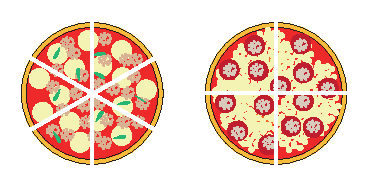
\includegraphics[scale=1.0]{pictures/Kuva3-1-6-pizzat.pdf}
        \end{center}

\begin{esimratk}
        Pizzan kokonaismäärän vertailua varten luvut on lavennettava samannimisiksi. Yhteiseksi nimittäjäksi tarvitaan luku, joka on jaollinen sekä kuudella että neljällä. Huomataan, että $12 = 3\cdot 4 = 2\cdot 6$. Murtolukujen nimittäjään tarvitaan siis luku $12$.
        Mintun saama määrä pizzaa on
        \begin{align*}
           \frac{2}{6} + \frac{1}{4} &= \frac{2\cdot 2}{2\cdot 6} + \frac{3\cdot 1}{3\cdot 4} \\ 
	       							 &= \frac{4}{12}+\frac{3}{12} \\ 
	       							 &= \frac{7}{12}.
        \end{align*}
        
        Vesan saama määrä pizzaa on
        \[
            \frac{2}{4} =
            \frac{3\cdot 2}{3\cdot 4} =
            \frac{6}{12}.
        \]
\end{esimratk}        
        \begin{esimvast}
        Koska $6/12 < 7/12$, Minttu saa enemmän.
        \end{esimvast}
    \end{esimerkki}